\documentstyle[12pt,psfig]{article}
\pagestyle{plain}

\setlength{\textwidth}{16 cm}
\setlength{\textheight}{26.0 cm}
\setlength{\topmargin}{0pt}
\setlength{\headsep}{0pt}
\setlength{\headheight}{0pt}
\renewcommand{\baselinestretch}{1.0}
\setlength{\parskip}{\medskipamount}

\hoffset=-1.8cm
\voffset=-0.8cm

\begin{document}

\section*{Task 1: The Euclidean Algorithm (GCD)}
\setcounter{section}{1}
\setcounter{subsection}{0}

The famous Euclidean algorithm is found in Book VII of the {\em Elements}.
The {\em Elements} was written in 300 B.C.~by the Greek mathematician
Euclid.
It is rumored that 
King Ptolemy,
having looked through the {\em Elements},
hopefully asked Euclid if there were not a shorter way to geometry,
to which Euclid severely answered:
``In geometry there is no royal road!''
Probably we should not blame the King for looking for short cuts,
for there are thirteen books in the {\em Elements}\,!
The books consist mainly of the mathematical knowledge amassed by Euclid,
and possibly some discoveries of his own.
The great achievement of Euclid is the beautifully systematic presentation
of material as an organic whole.
The {\em Elements} remained a standard work for over two thousand years.
(see Episodes from the Early History of Mathematics, Asger Aaboe)

The modern Euclidean algorithm
is often presented as
\begin{enumerate}
\item	Let $A$ and $B$ be integers with $A > B \geq 0$.

\item	If $B = 0$,
	then the gcd is $A$ and the algorithm ends.

\item	Otherwise,
	find $q$ and $r$ such that
\[
A = q B + r	\mbox{\ where\ } 0 \leq r < B
\]

	Note that we have $0 \leq r < B < A$
	and $\gcd(A,B) = \gcd(B,r)$.
	Replace $A$ by $B$,
	$B$ by $r$.
	Go to Step 2.
\end{enumerate}
But the original Euclidean algorithm uses
subtraction instead of division.
It is based on the observation that
a common divisor of the positive integers $A$, $B$ is also a common
divisor of the integers $\min(A,B)$, $\max(A,B)-\min(A,B)$.
Thus the gcd of two positive integers can be found as
\begin{enumerate}
\item	Let $A$ and $B$ be {\bf positive} integers.

\item	If $A = B$ then the gcd is $B$ and the algorithm ends.

\item	Otherwise,
	replace $A$ by $\max(A,B)-\min(A,B)$,
	$B$ by $\min(A,B)$.
	Go to Step 2.
\end{enumerate}

For example, given $A = 24, B = 15$,
the original Euclidean algorithm produces
\begin{enumerate}
\item	$A = 24-15 = 9$, $B = 15$
\item	$A = 15-9 = 6$, $B = 9$
\item	$A = 9-6 = 3$, $B = 6$
\item	$A = 6-3 = 3$, $B = 3$
\end{enumerate}
That is,
before finding $\gcd(24,15) = 3$,
the original Euclidean algorithm has to execute Step 3 four times.

\clearpage

\subsection{Requirements}

Code a program that reads two positive integers
and writes an integer which is
the number of times
the original Euclidean algorithm
executes Step 3
before obtaining the gcd of the given integers.

\subsection{Input File {\tt GCD.IN}}

The file consists of one line containing two positive integers
(each not larger than 32767)
separated by one or more spaces.
A sample input file for the above example is
\begin{verbatim}
24 15
\end{verbatim}

\subsection{Output File {\tt GCD.OUT}}

The file consists of one line containing one
integer.
A sample output file for the above example is
\begin{verbatim}
4
\end{verbatim}

\newpage

\section*{Task 2: Scout Outing (SCOUT)}
\setcounter{section}{2}
\setcounter{subsection}{0}

You are the scout-master and are planning a hike at Pulau Udang.
There are $N (2 \leq N \leq 100)$ stations and the travel time
(a positive integer value $\leq 100)$ between two stations is made
known to everybody.

The stations are numbered from 1 to $N$.
The diagram below shows an example with $N = 8$ stations.

\begin{center}
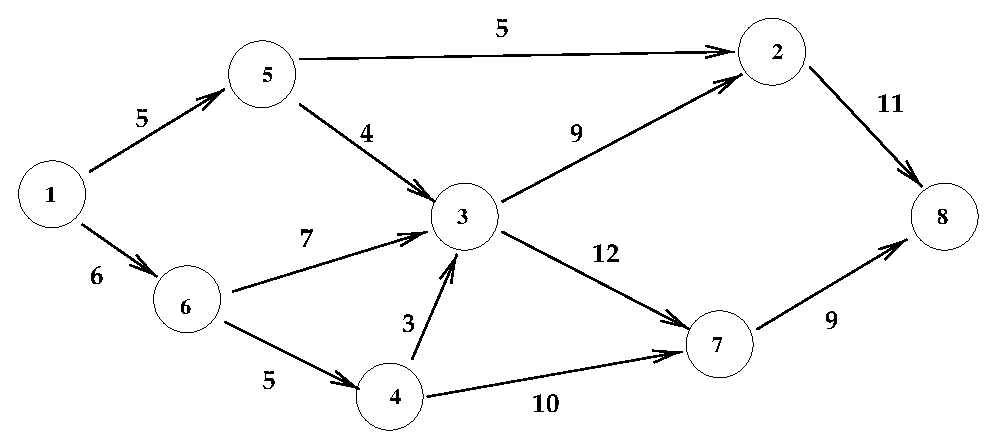
\psfig{file=scout.eps,height=2in,width=5in}
\end{center}

Everybody must start at station 1 and go through some path to arrive at
station $N$.
At each forked junction,
the scouts must split at the same
time to proceed to each of the forked routes.  For example, at station
1, the group is split into two --- one explores the route leading to
station 5, and the other proceeds to station 6.  The group that arrives
at station 5 must split into two again, one to go to station 2 and the
other to head for station 3.  In other words, no trail is left
unexplored.
A route has been fixed for each scout so that there are always
enough people to split up into the required number of groups,
and your routing plan is made known to everybody.

To ensure safety,
if a group arrives at a station earlier than other groups,
the early group must wait for the rest, until all have arrived
safely, before they split to proceed on at the same time.  
For example,
assuming that you start at time zero,
the earliest group
arrives at station 3 at time 9 (via station 5), and they have to wait
for the other two groups coming from station 6 and station 4.  When all
the 3 groups have arrived, they split into 2 groups and head for
stations 2 and 7.

Note that there is only one overall start station (at
station 1) and one overall end station (at station $N$),
every station is reachable from station 1,
and station $N$ is reachable from all the stations.
There is no cycle (otherwise you will go round and round!)

\subsection{Requirements}

You are to compute the earliest time $T$ when the last group can reach
station $N$,
assuming that the scouts start at time zero.
In the above example,
$T = 35$.
That is,
the earliest time for the last group to reach the final station 8 is 35.

Since a group that arrives at a station must wait for the other group(s)
to arrive before setting off again, this constitutes the waiting time. 
Formally, the waiting time at a station
is the duration between the arrival times of the first and the last groups
at that station.
For example, at station 3, the first group arrived at time 9
(via station 5), and the last group arrived at time 14 (via stations 6
and 4), so the waiting time at station 3 is 5.  Similarly, the waiting
time at station 2 is 13. 

You are to compute the total waiting time,
which is the sum of waiting times at all the stations,
for the whole trip.
In our example,
the total waiting time is  24.

At some stations, there is no need for the scouts to set off right away
after all the groups have arrived there.
They may actually take a rest and still
would not arrive at station $N$ later than time $T$.
For example, at station 5, the groups arrived at time 5, but can rest
until time 10 before setting off, without affecting $T$,
the earliest arrival time of the last group at station 8.
Similarly, when all groups have arrived at station 2,
they can rest for a further 1 unit of time.  However, at all the other
stations, the scouts must set off immediately without delay.
Hence, for our example, there are two stations (stations 5 and 2) where
the scouts may delay their departure.  

You are to compute how many stations there are at which delayed departure
is permitted.

\subsection{Input File {\tt SCOUT.IN}}

The file includes the integer $N (2\leq N\leq 100$, the number of stations)
and the integer $M (1\leq M\leq 1000$, the number of edges)
on the first line,
followed by
$M$
lines each containing 3 integers: the start station, the end station,
and the time to travel from the start station to the end station.  All
values are separated by one or more spaces.  The whole trip starts from
station 1 at time zero, and ends at station $N$.
For example:
\begin{verbatim}
8 12
3 7  12
5 2   5
6 3   7
1 6   6
4 7  10
2 8  11
1 5   5
5 3   4
6 4   5
7 8   9
4 3   3
3 2   9
\end{verbatim}

\subsection{Output File {\tt SCOUT.OUT}}

The output file should contain 3 integers,
separated by a space,
in a single line:
(1) the earliest time $T$ when the last group arrives at the final station $N$,
(2) the total waiting time,
and (3)
the number of stations where delayed departure is permitted.
For our example:

\begin{verbatim}
35 24 2
\end{verbatim}

\subsection{Marks}

Equal marks are allocated to these 3 output values.

\newpage

\section*{Task 3: Shortest Time Move (MOVE)}
\setcounter{section}{3}
\setcounter{subsection}{0}

The Sea of Sword Coast region can be divided into $n\times n$ regions
$(1 \leq n \leq 50)$.
Each region has different oceanic characteristics.
>From a region,
a ship can only move to its north, south, east, or west neighbor (if any).
The time needed to move from one region to a neighboring one depends
only on the destination region.
This duration is represented by a positive integer which is at most 1000. 
For example,
if $t[4,4]=10$,
then it takes 10 hours from each of the regions
$(3,4)$, $(5,4)$, $(4,5)$, or $(4,3)$
to move to region $(4,4)$.

Turning during the Sea Travel is not easy.
Sailors need to handle the change of the wind direction.
Ships also need to slow down first and gain momentum later.
It is mysterious but true,
if a ship is already moving in one particular direction,
it will take exactly 3 hours to change course.
For example, if t[4,4]=10 and t[4,5]=20,
then it takes 30 hours to sail the regions (4,3), (4,4), (4,5);
but it takes 3 more hours, or 33 hours, to sail regions
(3,4), (4,4), (4,5).

\begin{center}
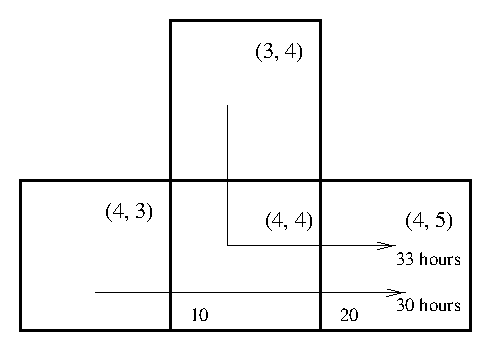
\psfig{file=move.eps,width=5cm,height=3cm}
\end{center}

\subsection{Requirements}

Now, the Mage Elminster is at region (1,1) and 
wishes, within the shortest time, to hurry to
the Baldur's Gate which is located at region ($n,n$).
Find what the shortest time is.
You must remember to include all turning times.

\subsection{Input File {\tt MOVE.IN}}

The first line of the file contains the integer $n$.
The cost array is given in the subsequent $n$ lines:
the second line contains the integers
$t[1,1]$, $t[1,2]$, $\cdots$, $t[1,n]$;
the third line contains the integers
$t[2,1]$, $t[2,2]$, $\cdots$, $t[2,n]$;
and so on;
finally the $(n+1)$-st line contains the integers
$t[n,1]$, $t[n,2]$, $\cdots$, $t[n,n]$.
Note that $t[1,1]$ is always 0.

For a $3\times 3$ Sword Coast, the 4 lines in the input file may look like: 
\begin{verbatim}
3
0 1 30
80 1 1
20 40 100
\end{verbatim}

\subsection{Output File {\tt MOVE.OUT}}
 
The file contains only one integer:
the minimum time that Elminster needs to reach Baldur's Gate.

For the example input file, the 1 line output file should be
\begin{verbatim}
112
\end{verbatim}

\newpage

\section*{Task 4: Rectangles (RECT)}

\setcounter{section}{4}
\setcounter{subsection}{0}

A rectangle whose edges are parallel to the axes can always be defined
by the two ends of one of its diagonals.
For example, a
rectangle can be drawn when the top left $(x_1, y_1)$ and the bottom right
$(x_2, y_2)$ coordinates are given.

\begin{center}
\begin{picture}(200,120)(0,0)
\put(25,25){\framebox(120,80){}}
\put(0,115){$(x_1,y_1)$}
\put(140,10){$(x_2,y_2)$}
\end{picture}
\end{center}

Given a set of rectangles, we are interested in finding the total area
covered by them.  For instance, the total area covered by the rectangles
below is the area covered within the solid lines.  Notice that
there is no double counting for overlapping regions.

\begin{center}
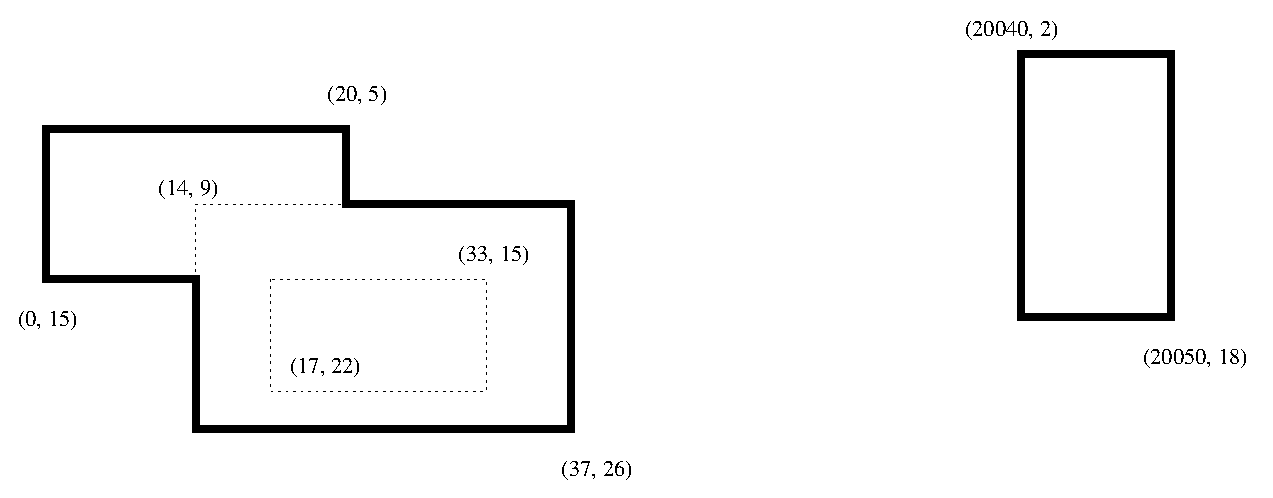
\psfig{file=rect4.eps,height=2.5in,width=5in}
\end{center}

\clearpage

\subsection{Requirements}

Write a program that, given a set of rectangles, computes the total area
covered by all the rectangles.

\subsection{Input File {\tt RECT.IN}}

The file describes a set of $N$ rectangles where $N$ ranges
between 0 to 1000.  On the first line is the integer $N$.  The remaining
lines are the coordinates of the rectangle.  In each of these line,
the two points $(x_1, y_1)$ and $(x_2, y_2)$ are given as 4 integers
$x_1, y_1, x_2, y_2$ separated by one or more blanks.
Note that they are NOT
necessarily the top-left and bottom-right coordinates.
In addition,
$x_i$ and $y_i$ take the value between 0 to $32767$.

For example,
the input file for the above example is
\begin{verbatim}
4
20 5 0 15
37 26 14 9
20040 2 20050 18
17 22 33 15
\end{verbatim}

\subsection{Output File {\tt RECT.OUT}}

On the first line of file , your program must write the
total area covered by the rectangles.
You may assume that the area is at most 32767.

For the above example,
the output file is
\begin{verbatim}
715
\end{verbatim}

\newpage

\section*{Task 5: Possible First Tiles (TILE)}

\setcounter{section}{5}
\setcounter{subsection}{0}

You are given a set of $M$
($1 \leq M \leq 10$)
$5 \times 5$ square tiles.
They are placed on an $N\times N$
($5 \leq N \leq 15$)
square table one at a time,
with their edges parallel to the edges of the table.
Tiles placed later might partially cover tiles placed earlier.
After the last tile is placed on the table,
the configuration can be represented by a top-view.
For example,
Top-view~1 denotes that tile A was placed after tile B on
a $11 \times 11$ square table.

\begin{center}
\begin{minipage}{1.5in}
Top-view 1
\begin{verbatim}
...........
..BBBBB....
..BBBBB....
..BBBBB....
..BBAAAAA..
..BBAAAAA..
....AAAAA..
....AAAAA..
....AAAAA..
...........
...........
\end{verbatim}
\end{minipage}
\begin{minipage}{1.5in}
Top-view 2
\begin{verbatim}
...........
..BBBBB....
..BBBBB....
..BBBBB....
..BBAAAAA..
..BBAAAAACC
DDDDAAAAACC
DDDDAAAAACC
DDDDAAAAACC
DDDDD.CCCCC
DDDDD......
\end{verbatim}
\end{minipage}
\begin{minipage}{1.5in}
Top-view 3
\begin{verbatim}
...........
...........
....AAAA...
...BAAAAB..
...BAAAAB..
...BAAAAB..
.CCCAAAAB..
.C.CCCCCB..
.CCCCCCC...
...........
...........
\end{verbatim}
\end{minipage}
\begin{minipage}{1.5in}
Top-view 4
\begin{verbatim}
...AAAAA...
...AAAAA...
...AAAAA...
...AAAAADDD
BBBBBAAADDD
BBBBB.DDDDD
BBBCCCDDDDD
BBBCCCDDDDD
BBBCCCCC...
...CCCCC...
...CCCCC...
\end{verbatim}
\end{minipage}
\end{center}

The tiles are named with consecutive letters beginning from A.
For example, if there are 5 tiles, then they will be called
A, B, C, D and E.
In a top-view,
each position on the table is represented
either by a ``.'' if that position is not covered
or a letter which is the name of the tile
that is top-most at that position.

If the given top-view is valid, it is possible to decide
a set of tiles each of which might have been the very first tile that
was placed on the table.
For example,
consider Top-view~2.
It is possible that tile B or C or D
is the first tile that was placed on the table.
However, it is impossible that A is the first tile
that was placed on the table.

There are two possible reasons that a top-view is invalid.
The first reason is that some tiles are not a $5 \times 5$ square.
For example, Top-view~3 is invalid:
A is a $4 \times 5$ tile,
the width of B exceeds 5,
and
C has a hole.
Any of these reasons is enough
to conclude that this top-view is invalid.

The second reason is that tiles could not have been placed one after another.
It is impossible that the tiles in Top-view 4 were placed one at a time ---
the four tiles are interlocking.
Hence, this top-view is invalid.

\clearpage

\subsection{Requirements}

Given a top-view, 
if it is invalid, you are to output the 2 letters ``NO''.
Otherwise, you are to output the 
letters in ascending order of the tiles each of which might be the first tile.
 
\subsection{Input File {\tt TILE.IN}}

The file contains the integer $M$, the number of tiles,
on the first line;
the integer $N$, the size of the $N\times N$ square table on the next line;
and then the top-view,
given as one row at each line.

Sample Input: 
\begin{verbatim}
4
15
...............
..BBBBB........
..BBBBB........
..BBBBB........
..BBAAAAA......
.CCCCCAAA......
.CCCCCAAA......
.CCCCCAAA......
.CCCCCAAA......
.CCCCC.........
...............
...............
...............
...............
...............
\end{verbatim}

\subsection{Output File {\tt TILE.OUT}}
 
The output file contains either the string ``NO'', or a
string of letters (in ascending order)
representing the possible first tiles.
There should be no spaces between the letters.
 
If a top-view is invalid, the output should be:
\begin{verbatim} 
NO
\end{verbatim}

For the above example, the output should be:
\begin{verbatim} 
BD
\end{verbatim}

\end{document}

